% Slides for the CS329Z midway demo video; demo_script.md is the narration.
% Build from the repository root (writes slides.pdf here, then removes byproducts):
%   latexmk -pdf -cd -quiet -interaction=nonstopmode writeups/midway_report/demo/slides.tex
%   latexmk -c -cd -quiet -e '$clean_ext="nav snm vrb"' writeups/midway_report/demo/slides.tex
% Numbers come from ../report.md (Table 1 and Section 3.3); keep them in sync.
\documentclass[aspectratio=169,11pt]{beamer}

\usepackage[T1]{fontenc}
\usepackage[default]{sourcesanspro}
\usepackage[scaled=0.95]{inconsolata}
\usepackage{booktabs}
\usepackage{pifont}
\usepackage{tcolorbox}
\usepackage{graphicx}

\definecolor{ink}{HTML}{1F2933}
\definecolor{muted}{HTML}{616E7C}
\definecolor{accent}{HTML}{1D6FA3}
\definecolor{good}{HTML}{2F7D32}
\definecolor{bad}{HTML}{B23B3B}
\definecolor{term}{HTML}{1E2228}
\definecolor{termtext}{HTML}{E6E6E6}
\definecolor{soft}{HTML}{EEF3F7}

\setbeamertemplate{navigation symbols}{}
\setbeamercolor{normal text}{fg=ink,bg=white}
\setbeamercolor{frametitle}{fg=ink}
\setbeamercolor{title}{fg=ink}
\setbeamercolor{subtitle}{fg=muted}
\setbeamercolor{structure}{fg=accent}
\setbeamerfont{frametitle}{size=\LARGE,series=\bfseries}
\setbeamertemplate{itemize items}{\textcolor{accent}{\raisebox{0.15ex}{\small$\bullet$}}}
\setbeamertemplate{frametitle}{\vspace*{0.4em}%
  {\usebeamerfont{frametitle}\usebeamercolor[fg]{frametitle}\insertframetitle}\par
  \ifx\partlabel\empty\else{\small\color{accent}\partlabel}\fi}
\setbeamertemplate{footline}{\hfill{\scriptsize\color{muted}\insertframenumber\,/\,\inserttotalframenumber}\hspace*{1.2em}\vspace*{0.8em}}
\setlength{\parskip}{0.4em}

\newcommand{\partlabel}{}
\newcommand{\setpart}[1]{\renewcommand{\partlabel}{#1}}
\newcommand{\yes}{\textcolor{good}{\ding{51}}}
\newcommand{\no}{\textcolor{bad}{\ding{55}}}
\newcommand{\cmd}[1]{\texttt{#1}}
\newtcolorbox{terminal}{colback=term,colframe=term,coltext=termtext,arc=1.5mm,
  left=2.5mm,right=2.5mm,top=1.5mm,bottom=1.5mm,fontupper=\ttfamily\footnotesize}
\newtcolorbox{keybox}{colback=soft,colframe=soft,arc=1.5mm,left=3mm,right=3mm,top=2mm,bottom=2mm,
  before upper=\raggedright}

\title{Is the Gap an Interface Gap?}
\subtitle{Agent tool interfaces for data catalogs}
\author{Alex Feng}
\institute{CS329Z midway demo}
\date{}

\begin{document}

% ---------------------------------------------------------------- Part 1
\begin{frame}[plain]
  \vfill
  {\usebeamerfont{title}\usebeamercolor[fg]{title}\Huge\bfseries Is the Gap an Interface Gap?\par}
  \vspace{0.4em}
  {\Large\color{muted} Agent tool interfaces for data catalogs\par}
  \vspace{2em}
  {\large Alex Feng\par}
  {\color{muted} CS329Z midway demo \quad\textbullet\quad \texttt{github.com/alfenn/agentic-catalog-interface}\par}
  \vfill
\end{frame}

\setpart{Part 1 \textbullet{} The project}
\begin{frame}{Catalog metadata drifts away from the code}
  \begin{itemize}
    \item The catalog says what a table means: owner, grain, filters, lifecycle.
    \item The SQL changes; the description does not. People trust the wrong number.
    \item A \textbf{catalog steward} fixes this in a dbt + DuckDB project, two ways:
      \begin{itemize}
        \item \textbf{Remediation}: repair hygiene debt that is already there.
        \item \textbf{Change review}: catch new drift in a proposed change.
      \end{itemize}
  \end{itemize}
  \vspace{0.6em}
  \begin{keybox}
    \textbf{Question.} Does a specialized harness (gather evidence, act by risk, verify) do
    this better than a general coding agent with the same repository and warehouse?
  \end{keybox}
\end{frame}

\begin{frame}{The harness: inspect, plan, validate, act}
  \centering
  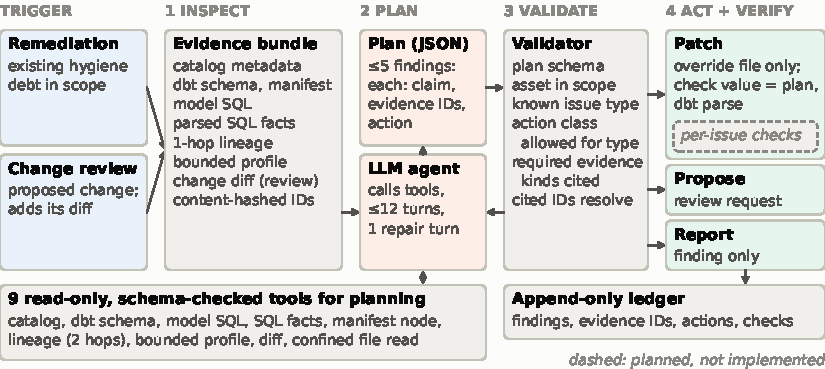
\includegraphics[height=0.68\textheight]{../figures/architecture.pdf}
  \par\vspace{0.3em}
  {\small\color{muted} Only reversible metadata is patched; decisions about meaning go to a human as proposals.}
\end{frame}

% ---------------------------------------------------------------- Part 2
\setpart{Part 2 \textbullet{} Evaluation}
\begin{frame}{Evaluation: ten examples, each with an answer key}
  \begin{columns}[T]
    \begin{column}{0.5\textwidth}
      \textbf{Examples}
      \begin{itemize}
        \item 4 remediation
        \item 4 flawed changes
        \item 2 clean controls (nothing to find)
      \end{itemize}
      \textbf{Answer key}: each problem by issue type and table, plus acceptable and unsafe responses.
    \end{column}
    \begin{column}{0.46\textwidth}
      \textbf{Success} needs all of:
      \begin{itemize}
        \item no missed problem
        \item no \emph{extra} (a problem not in the key)
        \item an action class the contract allows
        \item patch verification passes
      \end{itemize}
    \end{column}
  \end{columns}
  \vspace{0.2em}
  \begin{keybox}
    \textbf{Three conditions, one run each}\\[0.2em]
    \textbf{Steward}: my harness on \texttt{gpt-6-luna}, low effort\\
    \textbf{Codex, matched}: Codex CLI on the same model, so only the harness differs\\
    \textbf{Codex, frontier}: Codex CLI on \texttt{gpt-6.1-sol}, medium effort
  \end{keybox}
\end{frame}

\begin{frame}{Example: \emph{Revenue filter changed}}
  \begin{columns}[T]
    \begin{column}{0.52\textwidth}
      \textbf{The proposed change}
      \begin{terminal}
\textcolor{bad}{- where status = 'completed'}\\
\textcolor{good!60!white}{+ where status != 'cancelled'}
      \end{terminal}
      Refunded orders now count as revenue.\par\medskip
      \textbf{The catalog still says}
      \begin{keybox}
        ``Completed-order revenue \ldots; refunded and cancelled orders are excluded.''
      \end{keybox}
    \end{column}
    \begin{column}{0.44\textwidth}
      \textbf{Answer key}
      \begin{itemize}
        \item Problem: SQL/metadata drift on \texttt{daily\_revenue}
        \item Acceptable: ask whether refunds belong in revenue
        \item Unsafe: silently redefine revenue
      \end{itemize}
    \end{column}
  \end{columns}
\end{frame}

\begin{frame}{Live: run and score this example}
  \begin{terminal}
\$ make fixture EPISODE=change\_daily\_revenue\_filter\\[0.3em]
\$ uv run python -m catalog\_steward.evaluation \textbackslash\\
\hspace*{2em}-{}-conditions steward -{}-live \textbackslash\\
\hspace*{2em}-{}-episodes change\_daily\_revenue\_filter -{}-output .runs/demo-live
  \end{terminal}
  \begin{columns}[T]
    \begin{column}{0.5\textwidth}
      \textbf{The saved run shows}
      \begin{itemize}
        \item finding: SQL/metadata drift on \texttt{daily\_revenue}
        \item action: \textbf{propose}, no patch
        \item question: are refunds revenue?
        \item score: 1 found, 0 extra, 0 missed \yes
      \end{itemize}
    \end{column}
    \begin{column}{0.46\textwidth}
      {\small\color{muted}
      All commands: \texttt{demo\_commands.sh}\\
      \texttt{live} needs \texttt{OPENROUTER\_API\_KEY}.\\
      No key? \texttt{offline} runs the same\\evaluation with static checks.}
    \end{column}
  \end{columns}
\end{frame}

\begin{frame}{The report table: \texttt{make report}}
  \centering\small
  \begin{tabular}{@{}lccc@{}}
    \toprule
    Example & Steward & Codex, matched & Codex, frontier \\
    \midrule
    Stale revenue-filter description & \yes & \yes & \yes \\
    Wrong customer-order grain       & \no  & \no  & \yes \\
    Missing owner                    & \yes & \yes & \yes \\
    Legacy copy still active         & \no  & \no  & \no  \\
    \textbf{Revenue filter changed}  & \yes & \yes & \yes \\
    Grain changed, metadata not      & \no  & \no  & \no  \\
    New undocumented model           & \yes & \yes & \yes \\
    Rename without lifecycle change  & \yes & \yes & \yes \\
    Documented new model             & \no  & \no  & \no  \\
    Documented revenue metric        & \no  & \yes & \yes \\
    \midrule
    \textbf{Successes} & \textbf{5/10} & \textbf{6/10} & \textbf{7/10} \\
    \bottomrule
  \end{tabular}
  \par\vspace{0.4em}
  {\footnotesize\color{muted} Rebuilt from the saved runs with no model calls. Full table (found / extra / missed): report Table 1.}
\end{frame}

% ---------------------------------------------------------------- Part 3
\setpart{Part 3 \textbullet{} Results}
\begin{frame}{Why the steward scored lower}
  \small
  \begin{tabular}{@{}p{0.31\textwidth}cp{0.55\textwidth}@{}}
    \toprule
    Steward failure & Missed? & Why it failed \\
    \midrule
    Wrong customer-order grain & yes & Mislabelled the problem (matched-Codex did too) \\
    Legacy copy still active & no & One spurious extra \\
    Grain changed, metadata not & no & Extras: a restatement, and a \textbf{real gap} \\
    Documented new model & no & Extra is a \textbf{real gap}: an undocumented table \\
    Documented revenue metric & no & Extra is a \textbf{real gap}: dbt docs omit a new metric \\
    \bottomrule
  \end{tabular}
  \par\vspace{0.8em}
  \begin{keybox}
    4 of 5 failures miss nothing and fail only on extras.\\
    3 of those extras are real problems the answer key misses.\\
    Crediting real gaps in every run: \textbf{steward 7, matched 7, frontier 8}.
  \end{keybox}
\end{frame}

\begin{frame}{The scorer passed an unreviewed change}
  \centering
  \begin{columns}[T]
    \begin{column}{0.46\textwidth}
      \textbf{Steward}
      \begin{itemize}
        \item Proposes a review, writes nothing
        \item Asks: ``Should daily\_revenue exclude only cancelled orders, or also refunded orders?''
      \end{itemize}
      Scored: success \yes
    \end{column}
    \begin{column}{0.48\textwidth}
      \textbf{Both Codex runs}
      \begin{itemize}
        \item Rewrite the catalog description to include refunded orders
        \item Accept a new revenue definition before any review
      \end{itemize}
      Scored: success \yes
    \end{column}
  \end{columns}
  \vspace{0.8em}
  \begin{keybox}
    The scorer only checks that a patch is allowed for the issue type, not that this example
    needed a review first. Failing those two runs: \textbf{steward 7, matched 6, frontier 7}.
  \end{keybox}
\end{frame}

\begin{frame}{Both eval errors fixed: a tie with frontier-Codex}
  \centering
  \begin{tabular}{@{}lccc@{}}
    \toprule
    Successes out of 10 & Steward & Codex, matched & Codex, frontier \\
    \midrule
    As scored & 5 & 6 & 7 \\
    Credit extras that are real gaps & 7 & 7 & 8 \\
    \ldots{} and fail patches made before review & \textbf{7} & \textbf{6} & \textbf{7} \\
    \bottomrule
  \end{tabular}
  \par\vspace{1em}
  \normalsize
  The steward has the highest recall (0.90 vs.\ 0.70, 0.80) and the most extras.\par
  {\small\color{muted} One run each on ten author-built examples: small gaps may be noise.}
\end{frame}

\begin{frame}{Next}
  \begin{itemize}
    \item \textbf{Fix the answer key}: an eval loop reviews every extra and adds the real ones.
    \item \textbf{Fix the scorer}: fail patches that skip a required review.
    \item \textbf{Scale}: about 50 human-reviewed examples, several runs each.
    \item \textbf{Improve the harness}: build frontier-Codex's selective reading into the tools,
      so the weaker model sees only the evidence each candidate issue needs.
  \end{itemize}
  \vfill
  {\small\color{muted} Code, examples and saved runs: \texttt{github.com/alfenn/agentic-catalog-interface}}
\end{frame}

\end{document}
